\documentclass{standalone}
\usepackage{tikz}

\definecolor{mBlue}{HTML}{22a1dc}
\definecolor{sBlue}{HTML}{009FE3}
\definecolor{sYellow}{HTML}{FFED00}
\definecolor{sRed}{HTML}{E30613}
\definecolor{sGreen}{HTML}{009640}
\definecolor{sPurple}{HTML}{440099}
\definecolor{mGreen}{HTML}{86cd30}
\definecolor{darkgreen}{HTML}{006400}
\definecolor{mLightBrown}{HTML}{e68a00}
\definecolor{lightred}{HTML}{FF9999}

%% COLOUR COMMANDS
\newcommand{\sBlue}[1]{\textcolor{sBlue}{#1}}
\newcommand{\sB}[1]{\sBlue{#1}}
\newcommand{\sRed}[1]{\textcolor{sRed}{#1}}
\newcommand{\sR}[1]{\sRed{#1}}
\newcommand{\sGreen}[1]{\textcolor{sGreen}{#1}}
\newcommand{\sG}[1]{\sGreen{#1}}
\newcommand{\sPurple}[1]{\textcolor{Purple}{#1}}
\newcommand{\sP}[1]{\sPurple{#1}}
\newcommand{\sYellow}[1]{\textcolor{sYellow}{#1}}
\newcommand{\sY}[1]{\sYellow{#1}}

\begin{document}
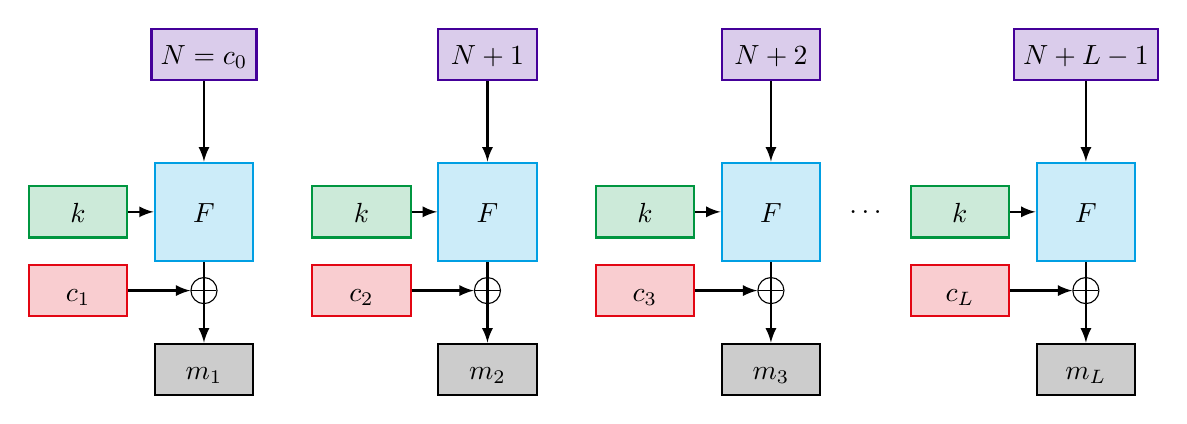
\begin{tikzpicture}[yscale=-1,xscale=0.8,>=latex]
		\tikzstyle{RECT} = [thick, minimum width=1.25cm, minimum height=0.65cm, text height=2ex, text depth=0.25ex]
		\tikzstyle{SQUA} = [thick, minimum width=1.25cm, minimum height =1.25cm, text height=2ex, text depth=0.25ex]
		\tikzstyle{key} = [RECT, draw=sGreen, fill=sGreen!20]
		\tikzstyle{prf} = [SQUA, draw=sBlue, fill=sBlue!20]
		\tikzstyle{tag} = [RECT, draw=sRed, fill=sRed!20]
		\tikzstyle{message} = [RECT, draw=black, fill=black!20]
		\tikzstyle{nonce} = [RECT, draw=sPurple, fill=sPurple!20]
		\tikzset{XOR/.style={draw,circle,append after command={
					[shorten >=\pgflinewidth, shorten <=\pgflinewidth,]
					(\tikzlastnode.north) edge (\tikzlastnode.south)
					(\tikzlastnode.east) edge (\tikzlastnode.west)
				}
			}
		}
		
		\node[tag] (mOne) at  	(-2, 3) {$c_1$};
		\node[nonce] (NOne) at (0,0)		{$N=c_0$};
		\node[XOR] (xOne) at (0,3)			{};
		\node[key] (kOne) at 		(-2, 2) {$k$};
		\node[prf] (pOne) at		(0, 2) {$F$};
		\node[message] (cOne) at		(0, 4) {$m_1$};
		\draw[->, thick] (mOne.east) -- (xOne.west);
		\draw[->, thick] (kOne.east) -- (pOne.west);
		\draw[->,thick] (pOne.south) -- (cOne.north); 
		\draw[->,thick] (NOne.south) -- (pOne.north);
		
		\node[tag] (mTwo) at  	(2.5, 3) {$c_2$};
		\node[nonce] (NTwo) at (4.5,0)	{$N+1$};
		\node[XOR] (xTwo) at (4.5,3) {};
		\node[key] (kTwo) at 		(2.5, 2) {$k$};
		\node[prf] (pTwo) at		(4.5, 2) {$F$};
		\node[message] (cTwo) at		(4.5, 4) {$m_2$};
		\draw[->, thick] (mTwo.east) -- (xTwo.west);
		\draw[->, thick] (kTwo.east) -- (pTwo.west);
		\draw[->,thick] (pTwo.south) -- (cTwo.north); 
		\draw[->,thick] (NTwo.south) -- (pTwo.north);

		\node[tag] (mThree) at  (7, 3) {$c_3$};
		\node[nonce] (NThree) at (9,0) {$N+2$};
		\node[XOR] (xThree) at (9,3) {};
		\node[key] (kThree) at 		(7, 2) {$k$};
		\node[prf] (pThree) at		(9, 2) {$F$};
		\node[message] (cThree) at		(9, 4) {$m_3$};
		\draw[->, thick] (mThree.east) -- (xThree.west);
		\draw[->, thick] (kThree.east) -- (pThree.west);
		\draw[->,thick] (pThree.south) -- (cThree.north); 
		\draw[->,thick] (NThree.south) -- (pThree.north);
		
		\node[tag] (mN) at  (12, 3) {$c_L$};
		\node[nonce] (NN) at (14,0) {$N+L-1$};
		\node[XOR] (xN) at (14,3) {};
		\node[key] (kN) at 		(12, 2) {$k$};
		\node[prf] (pN) at		(14, 2) {$F$};
		\node[message] (cN) at		(14, 4) {$m_L$};
		\draw[->, thick] (mN.east) -- (xN.west);
		\draw[->, thick] (kN.east) -- (pN.west);
		\draw[->,thick] (pN.south) -- (cN.north); 
		\draw[->,thick] (NN.south) -- (pN.north);

		\node[] (dots) at (10.5,2) {$\ldots$};
\end{tikzpicture}
\end{document}
